\documentclass{article}
\usepackage[utf8]{inputenc}
\usepackage[T1]{fontenc} % Recomendado para documentos en español
\usepackage{graphicx}
\usepackage[spanish,es-tabla]{babel}
\usepackage{amsmath}
\usepackage[a4paper,margin=1in]{geometry}
\usepackage{subcaption}
\usepackage{amssymb}
\usepackage{mathtools}
\usepackage[table,xcdraw]{xcolor}
\usepackage{enumitem}
\usepackage{csquotes}
\usepackage[siunitx, american]{circuitikz}
\usepackage{newtxtext} % Tipografía Times New Roman
\usepackage{titlesec}  % Formato de títulos
\usepackage{standalone}
\usepackage{multicol}
\usepackage{multirow}
\usepackage[colorlinks=true, linkcolor=black, citecolor=black, urlcolor=black, filecolor=black]{hyperref}
\usepackage{cleveref}
\usepackage{float}
\usepackage[backend=biber, style=numeric]{biblatex} % Carga el paquete compatible con biber
\addbibresource{bibliografia.bib} % Vincula el archivo que acabas de crear
\usepackage{url}
\usepackage{listings}
\lstset{
  basicstyle=\ttfamily\small,
  breaklines=true,
  postbreak=\mbox{\textcolor{black}{$\hookrightarrow$}\space}
}

% Definición de tamaños exactos
\newcommand{\sizedieciocho}{\fontsize{18}{22}\selectfont}
\newcommand{\sizedieciseis}{\fontsize{16}{20}\selectfont}
\newcommand{\sizecatorce}{\fontsize{14}{18}\selectfont}
\newcommand{\sizedoce}{\fontsize{12}{16}\selectfont}

% Formato de títulos
\titleformat{\section}{\normalfont\sizedieciocho\bfseries}{}{0pt}{}
\titleformat{\subsection}{\normalfont\sizedieciseis\bfseries}{}{0pt}{}
\titleformat{\subsubsection}{\normalfont\sizecatorce\bfseries}{}{0pt}{}

% Indentación y espacios de títulos
\titlespacing*{\section}{0pt}{14pt}{8pt}
\titlespacing*{\subsection}{0.5cm}{12pt}{6pt}
\titlespacing*{\subsubsection}{1.0cm}{10pt}{4pt}

% Configuración de referencias automáticas
\crefname{figure}{Fig.}{Figuras}
\crefname{table}{Tab.}{Tablas}
\crefname{equation}{Ec.}{Ecuaciones}

% Configuración de referencias con autoref (para \autoref{})
\renewcommand{\figureautorefname}{Fig.}
\renewcommand{\tableautorefname}{Tab.}
\renewcommand{\equationautorefname}{Ec.}

\setcounter{secnumdepth}{0} % Sin numeración en títulos
\setcounter{tocdepth}{3}    % Muestra hasta sub-subsecciones en el índice

\begin{document}
\begin{titlepage}

\thispagestyle{empty}

% Portada Custom, ver /maketitle: https://www.overleaf.com/learn/latex/How_to_Write_a_Thesis_in_LaTeX_(Part_5)%3A_Customising_Your_Title_Page_and_Abstract

\begin{tikzpicture}[remember picture,overlay]
    \node[opacity=0.2,anchor=center] at (current page.center) 
        {
\includegraphics[width=0.9\paperwidth]{Imagenes/decoracion_a.png}};
\end{tikzpicture}

\begin{center}
    
\includegraphics[width=15cm]{Imagenes/unc_fcefyn_logo.png}
    \\[0.5cm]
    \LARGE Universidad Nacional de Córdoba\\[0.5cm] 
    \large Facultad de Ciencias Exactas, Físicas y Naturales \\[0.5cm] 
    \large Electrónica Analógica 1
    \\[0.2cm]
    \large Trabajo Práctico N° 3
    \\[0.2cm]
    \vspace{60pt}
    \begin{table}[!h]
    \centering
    \begin{tabular}{ll}
    \multicolumn{1}{c}{Nombre} & \multicolumn{1}{c}{DNI} \\
    Castilla, Juan Felipe & 45.886.652 \\
    Dalmazzo, Agustín Eduardo & 46.541.615 \\
    López Bernal, Julián & 45.107.175
    \end{tabular}
    \end{table}
    \vspace{20pt}
    \begin{table}[!h]
    \centering
    \begin{tabular}{ll}
    \multicolumn{1}{c}{Docentes} & Prof. Dadam, Federico Tomás \\
     & Prof. Gallardo, Fernando José \\
     & Prof. Petrashin, Pablo Antonio \\
    \end{tabular}
    \end{table}
    \vfill
    Córdoba, República Argentina\\
    \today
\end{center}

\end{titlepage}
\newpage
\vspace*{\fill} 
\newpage
\tableofcontents
\newpage
\listoffigures
\newpage
\listoftables
\newpage
\section{Introducción}

En este informe se explicará el proceso de diseño, fabricación y simulación de un amplificador de dos etapas con transistores MosFet. Los objetivos principales del trabajo son:

\begin{itemize}
  \item Ganancia mayor a 6
  \item Calcular Chf para una frecuencia de corte en alta de 20 kHz
\end{itemize}

Se detallarán a rasgos generales los procesos seguidos para cada uno de estos puntos y el contexto en el que se calculan, se cita además un repositorio (\cite{Repositorio}) en el cual se encontrará información adicional y todos los cálculos realizados, y se mostrarán los resultados tanto de diseño como simulación y medición del circuito real, para verificar el cumplimiento de los objetivos.
\section{Marco Teórico}

\subsection{Polarización de MosFets}

La curva de transferencia en los MosFets sigue la ecuación \ref{transferencia}, lo cual presenta una cierta dificultad a la hora de hacer el cálculo de polarización, ya que la corriente de salida no depende linealmente de la tensión de polarización. Es por esto que, como se discutirá en el diseño, se optó por resolver los circuitos por computadora.

\begin{equation}
  I_{DS} = K\cdot (V_{GS} - V_TH)^2
  \label{transferencia}
\end{equation}

Para hacer un modelado correcto del amplificador y poder resolverlo es necesario encontrar las ecuaciones que relacionen los parametros $V_{GS}$, $I_{DS}$ y $V_{DS}$ de cada transistor en el circuito (\ref{Amplificador Completo}).

\begin{figure}[H]
  \centering
  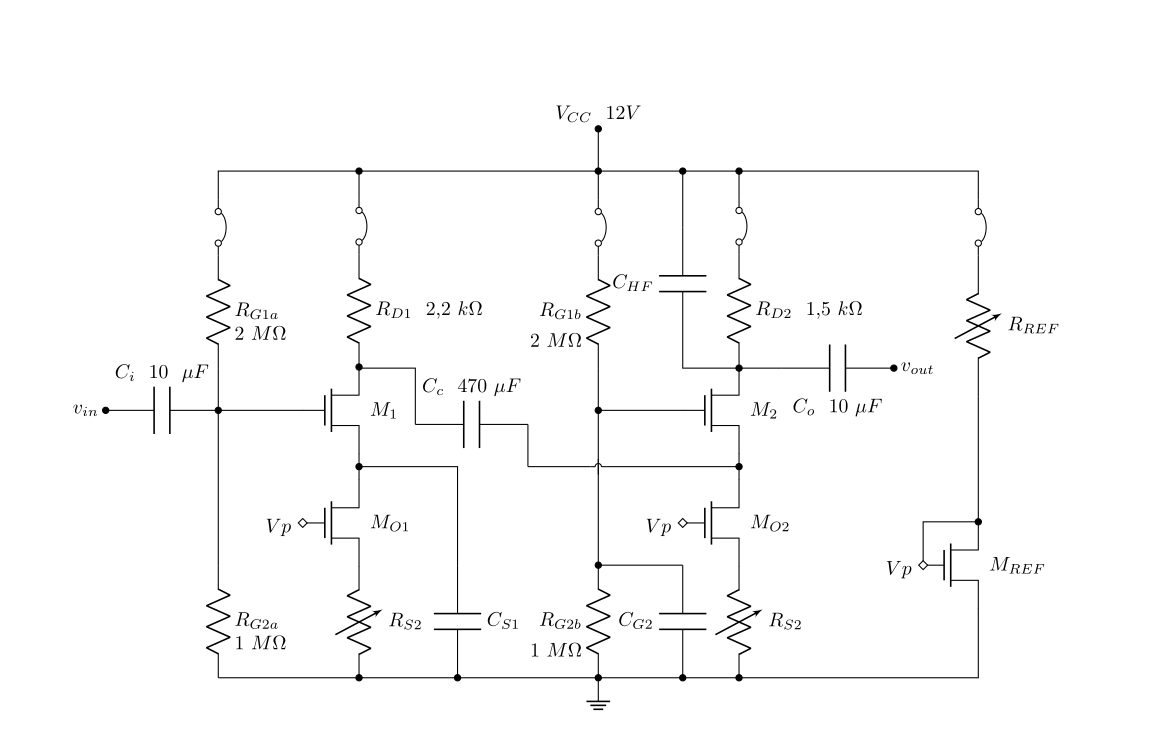
\includegraphics[width=\linewidth]{Imagenes/EsquematicoCatedra.png}
  \caption{Amplificador Completo}
  \label{Amplificador Completo}
\end{figure}

Encontrar esas relaciones implica conocer la relación entrada-salida de cada transistor ($V_{GS}$-$I_{DS}$) y la característica de salida ($I_{DS}$-$V_{DS}$), haciendo el análisis de mallas para encontrar las ecuaciones y poder calcular el punto de operación y las rectas de carga de los transistores.

El amplificador consta de dos etapas identicas en configuracón Fuente Común polarizadas con fuente de corriente (los transistores $M_{o1}$ y $M_{o2}$), por lo tanto, las rectas de carga solo se trazan para $M_{1}$ y $M_{2}$, ya que son estos los transistores amplificadores.

\subsubsection{Espejos de corriente}

La polarización con fuentes de corriente se logra con los espejos de corriente, que en este caso es fabricado con $M_{ref}$ y $R_{ref}$. Este transistor opera en una condición particular de polarización ($V_D = V_G$) y es polarizado únicamente por la resistencia $R_{ref}$. La $V_P = V_{Dref} = V_{Gref}$ es la tensión de polarización de $M_{o1}$ y $M_{o2}$ y es esto lo que forma el espejo de corriente. 

La corriente de $M_{ref}$ está fijada por $R_{ref}$, pero se relaciona con las corrientes de polarización de $M_{o1}$ y $M_{o2}$ (y, por consecuencia, de $M_{1}$ y $M_{2}$) con las resistencias variables de estos transistores. Esto permite lograr dos cosas, utilizar una fuente de corriente para polarizar los transistores amplificadores, lo que brinda una mayor estabilidad del punto Q, y modificar la ganacia total del amplificador variando un solo parámetro, $R_{ref}$.

La transconductancia de los MosFets es directamente proporcional a la corriente de drenaje, por lo que variando $R_{ref}$ es posible ajustar el valor de $I_{DSref}$, lo cual no tiene efecto directo en la ganancia, pero esto también varía las fracciones reflejadas de esta corriente en $M_{o1}$ y $M_{o2}$, que también son las de los transistores $M_{1}$ y $M_{2}$, que si tienen efecto en la ganancia. 

\subsection{Respuesta en Frecuencia}

El análisis de la ganancia se hace utilizando el modelo en pequeña señal de los transistores y considerando que el amplificador está operando en la banda media o de paso, donde los capacitores de baja frecuencia se comportan como cortocitcuito y los de alta frecuencia como un circuito abierto.

El cálculo y análisis de los capacitores de baja frecuencia se hace con este mismo modelo, para encontrar las frecuencias de corte de los capacitores se deben hacer algunas consideraciones antes de poder calcularlos. Se considera que un capacitor no tiene efecto sobre el resto cuando la frecuencia de su polo está alejada del resto en al menos tres octavas, idealmente una década, en estas condiciones es posible disernir el estado (alta o baja impedancia) del resto de capacitores con respecto al analizado.

En ocasiones, los capaciores del circuito están en mallas aisladas, por lo que no interactúan entre si y no es necesario tener esto en cuenta, en otros casos si están en la misma malla, por lo que, o se hace un análisis cualitativo previo para estimar cúal de los capacitores tendrá asociada una resistencia equivalente menor (este será el polo dominante) para disernir las condiciones del resto, o se tienen en cuenta todos los casos posibles y se anañizan los resultados de las frecuencias de corte para definir cuál es la condición correcta.

En el caso de baja frecuencia, los ceros se calculan como el inverso del producto entre el valor de capacitancia y la impedancia directamente asociada en paralelo, si esta no existe, como es el caso en los capacitores de desacoplo, esa impedancia es infinita y la frecuencia de corte es cero. Los polos se calculan como el inverso del producto entre la capacidad y la resistencia equivalente desde el capacitor analizado (equivalente de Thevenin).

El modelo en pequeña señal no alcanza para analizar el comportamiento en alta frecuencia del amplificador, ya que cobra relevancia el efecto de las capacidades parásitas de los transistores, por lo que es necesario considerarlas. Estas capacidades traen cosigo el efecto Miller, la reducción del ancho de banda a causa de una capacidad equivalente mayor a la parásita, dando una frecuencia de corte menor.

Si bien el modelo es distinto, la frecuencia del polo se calcula de la misma forma que en baja frecuencia, la distinción es que no hay ceros que contribuyan en alta frecuencia. En la función de transferencia las contribuciones de los ceros y polos en baja se expresan como $s + \omega_{Z}$ y $s + \omega_{P}$ y las de alta frecuencia como $1 + \frac{s}{\omega_{P}}$. La función de trasferencia de este amplificador se puede escribir como:

\begin{equation}
  A_{V}(s) = \frac{A_V \cdot s^3}{(s + \omega_{Co}) \cdot (s + \omega_{Cc}) \cdot (s + \omega_{Cs1}) \cdot (1 + \frac{s}{\omega_{Chf}})}
\end{equation}

La ausencia de $C_i$ y del posible polo en alta frecuencia generado por $M_1$ es debido a que, para simplificar el análisis, solo se tuvieron en cuenta las contribuciones en alta frecuencia de la última etapa, ya que el objetivo de $C_{hf}$ es limitar el ancho de banda, por lo que las contribuciones del capacitor parásito en alta de $M_1$ serían despreciables. Por otro lado, la resistencia equivalente de $C_i$ haría que su polo fuera despreciable, por lo que tampoco se tuvieron en cuenta sus contribuciones.




















\section{Desarrollo}

\subsection{Simulación Integral, Análisis Global del Amplificador}

\subsubsection{Esquemático y Caracterización General}
\begin{figure}[H]
    \centering
    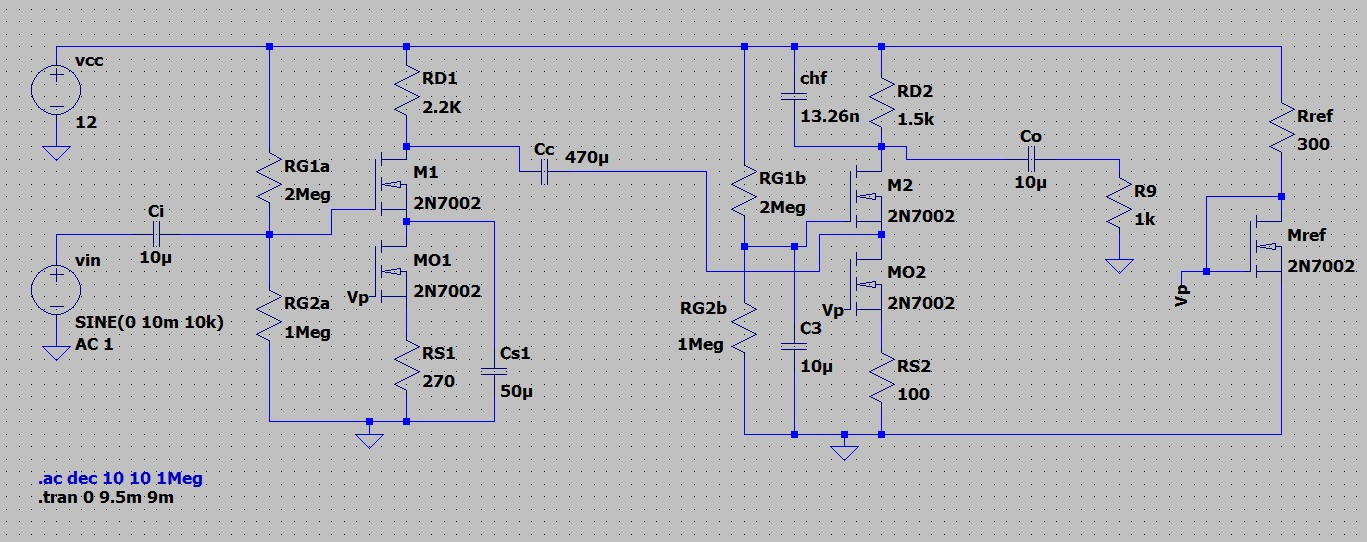
\includegraphics[width=0.85\linewidth]{Simu-Feli/Fotos/Spice-completo.jpg}
    \caption{Esquemático completo del amplificador MOSFET de 2 etapas en LTspice.}
    \label{fig:circuito_global}
\end{figure}

\subsubsection{Ganancia y Ancho de Banda}
\begin{figure}[H]
    \centering
    \begin{minipage}{0.48\textwidth}
        \centering
        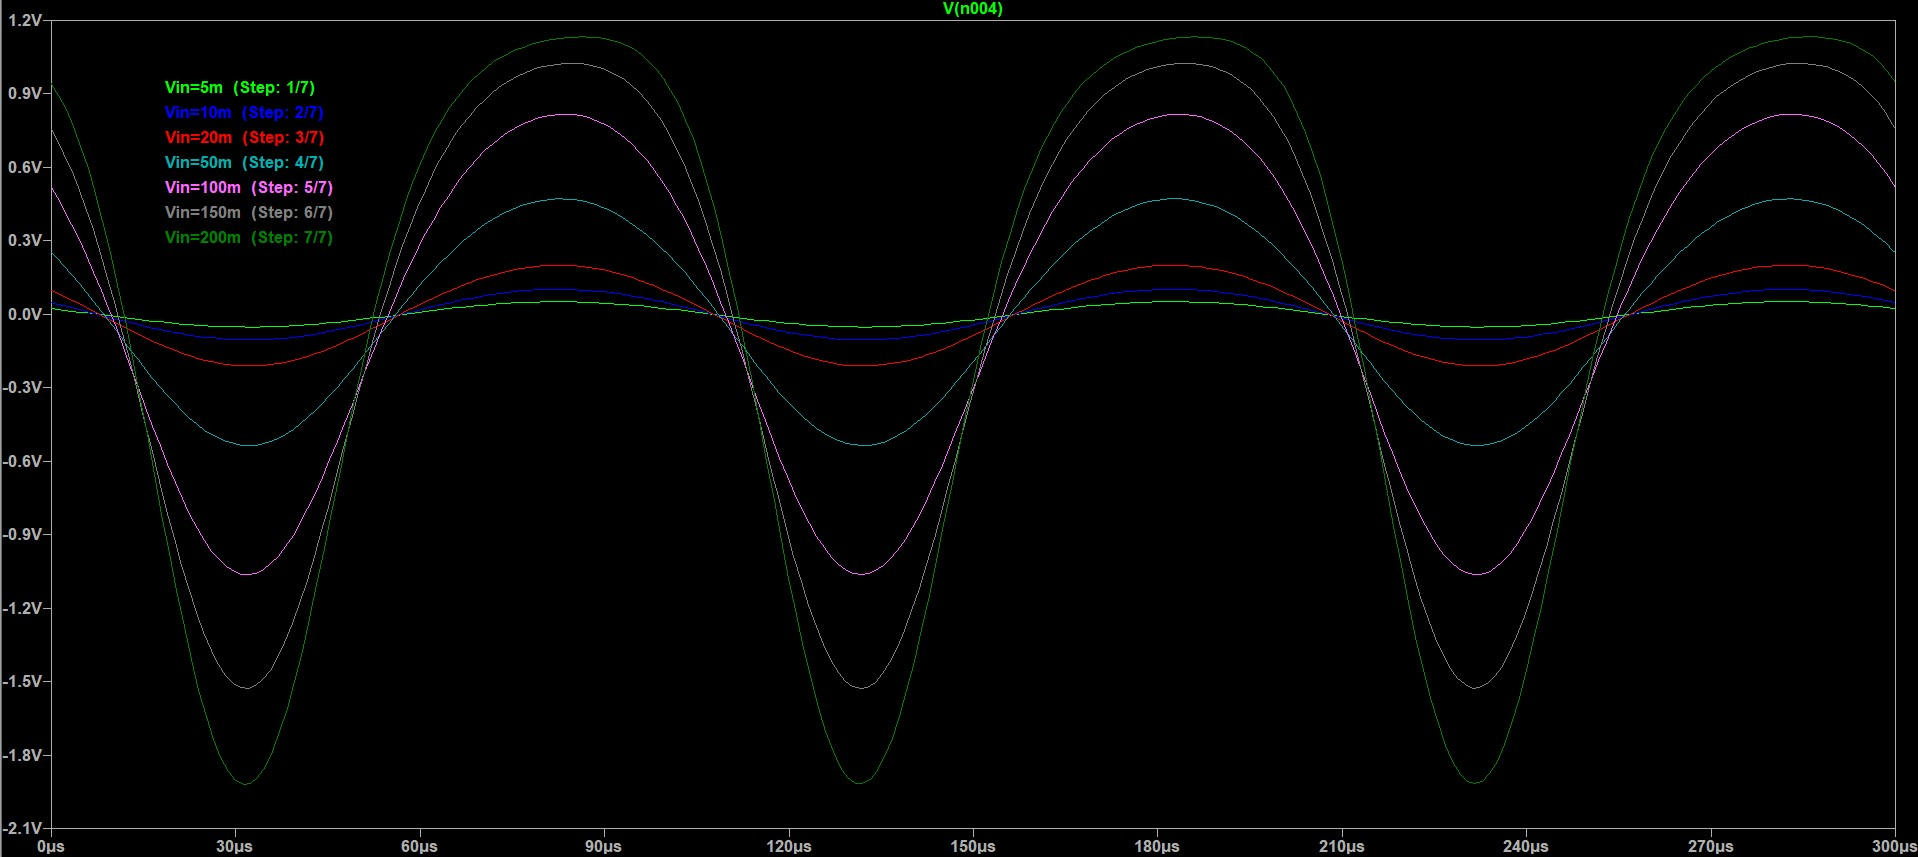
\includegraphics[width=\linewidth]{Simu-Feli/Fotos/Barrido_Vin_voltaje.jpg}
        \caption{Ganancia transitoria.}
    \end{minipage}\hfill
    \begin{minipage}{0.48\textwidth}
        \centering
        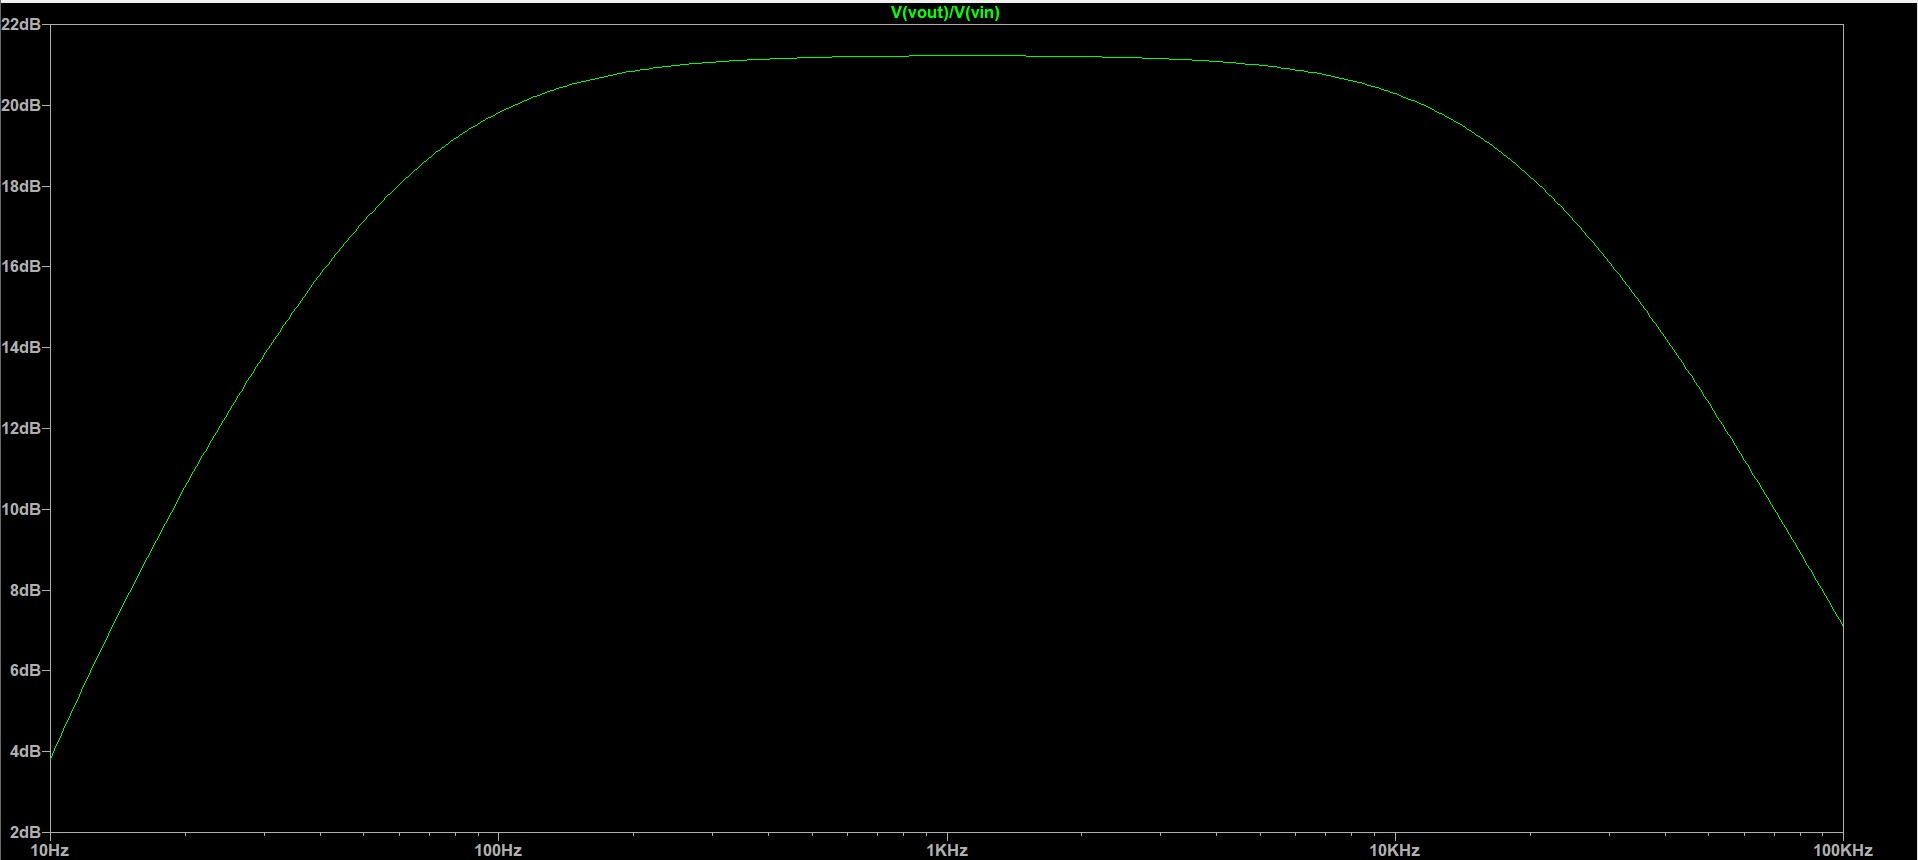
\includegraphics[width=\linewidth]{Simu-Feli/Fotos/Av_total.jpg
}
        \caption{Ganancia de tensión total $A_v$.}
    \end{minipage}
\end{figure}

\begin{figure}[H]
    \centering
    \begin{minipage}{0.48\textwidth}
        \centering
        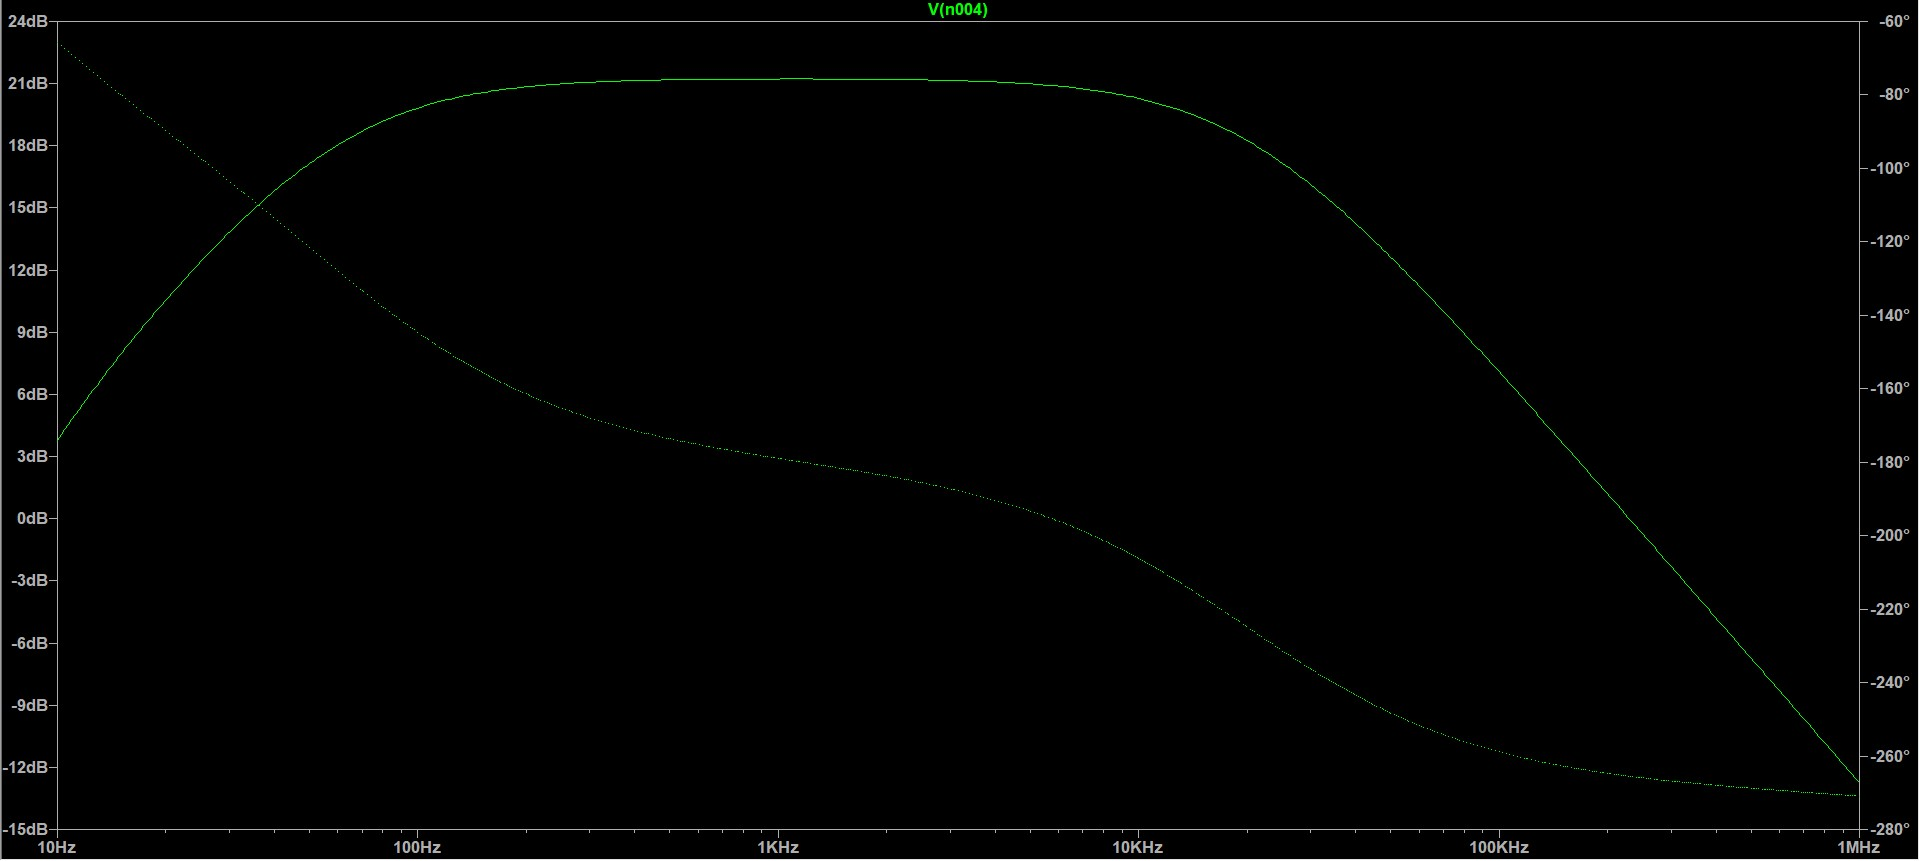
\includegraphics[width=\linewidth]{Simu-Feli/Fotos/BW-ConChf.jpg
        }
        \caption{Ancho de banda con $C_{hf}$.}
    \end{minipage}\hfill
    \begin{minipage}{0.48\textwidth}
        \centering
        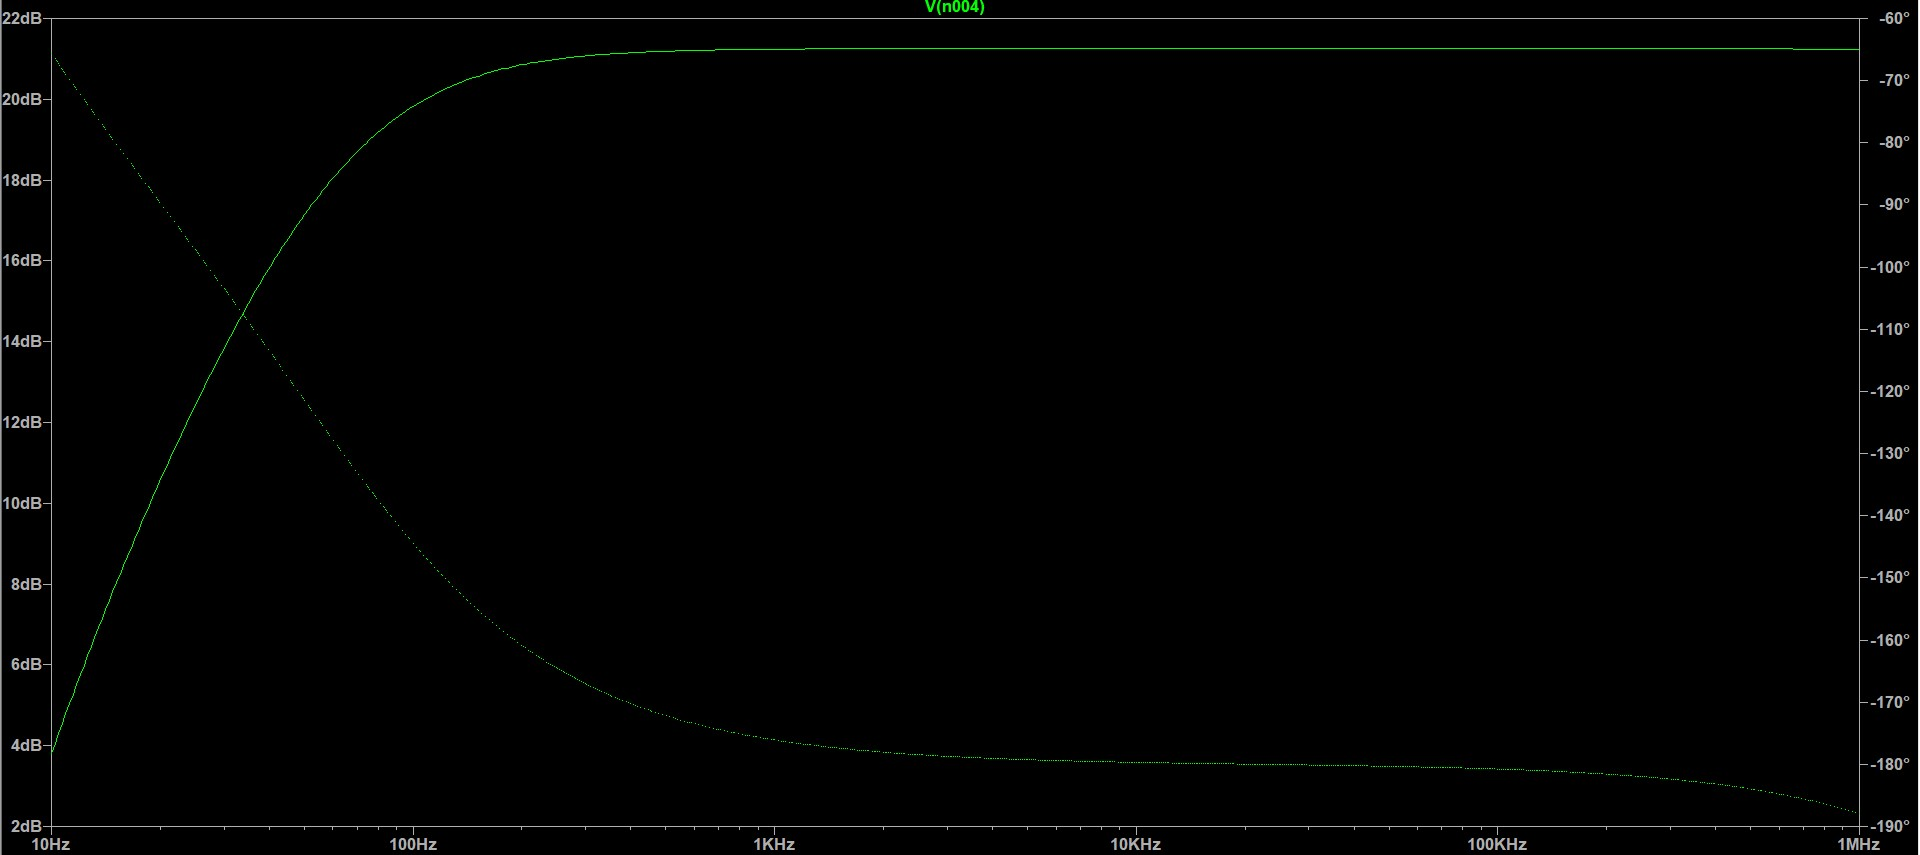
\includegraphics[width=\linewidth]{Simu-Feli/Fotos/BW-SinChf.jpg}
        \caption{Ancho de banda sin $C_{hf}$.}
    \end{minipage}
\end{figure}

\subsubsection{Impedancias Globales ($Z_{in}$ y $Z_{out}$)}
\begin{figure}[H]
    \centering
    \begin{minipage}{0.48\textwidth}
        \centering
        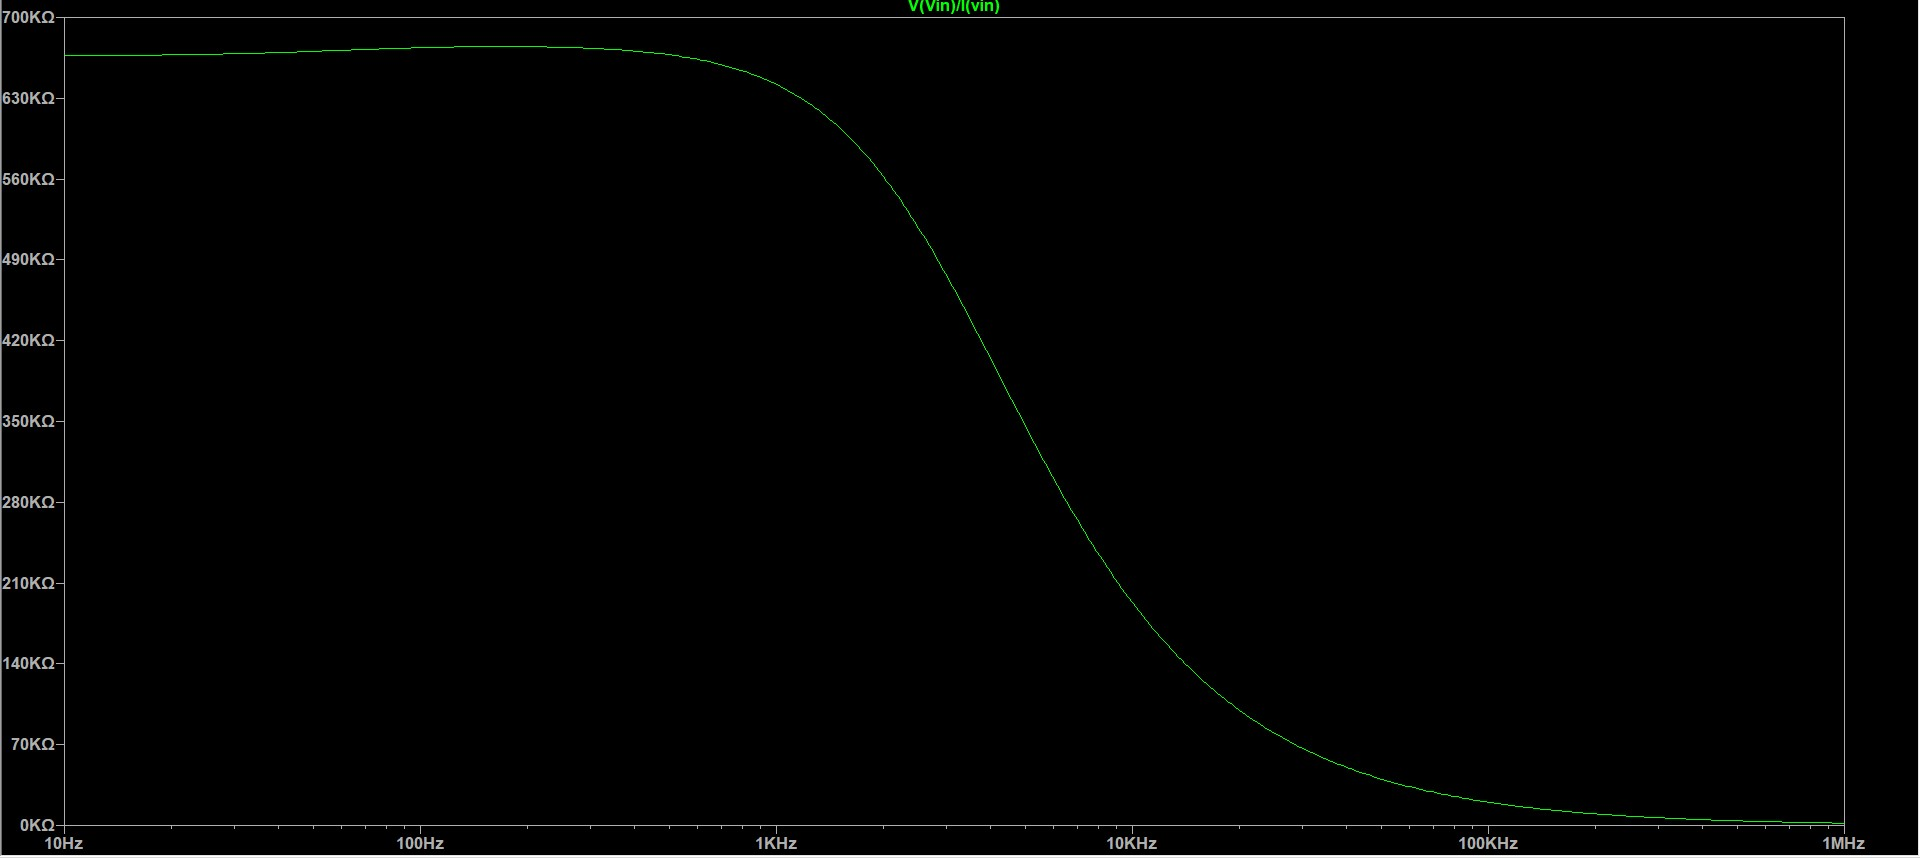
\includegraphics[width=\linewidth]{Simu-Feli/Fotos/Impedancia_In_TOAL.jpg}
        \caption{Montaje de medición de la impedancia de entrada total $Z_{in}$.}
    \end{minipage}\hfill
    \begin{minipage}{0.48\textwidth}
        \centering
        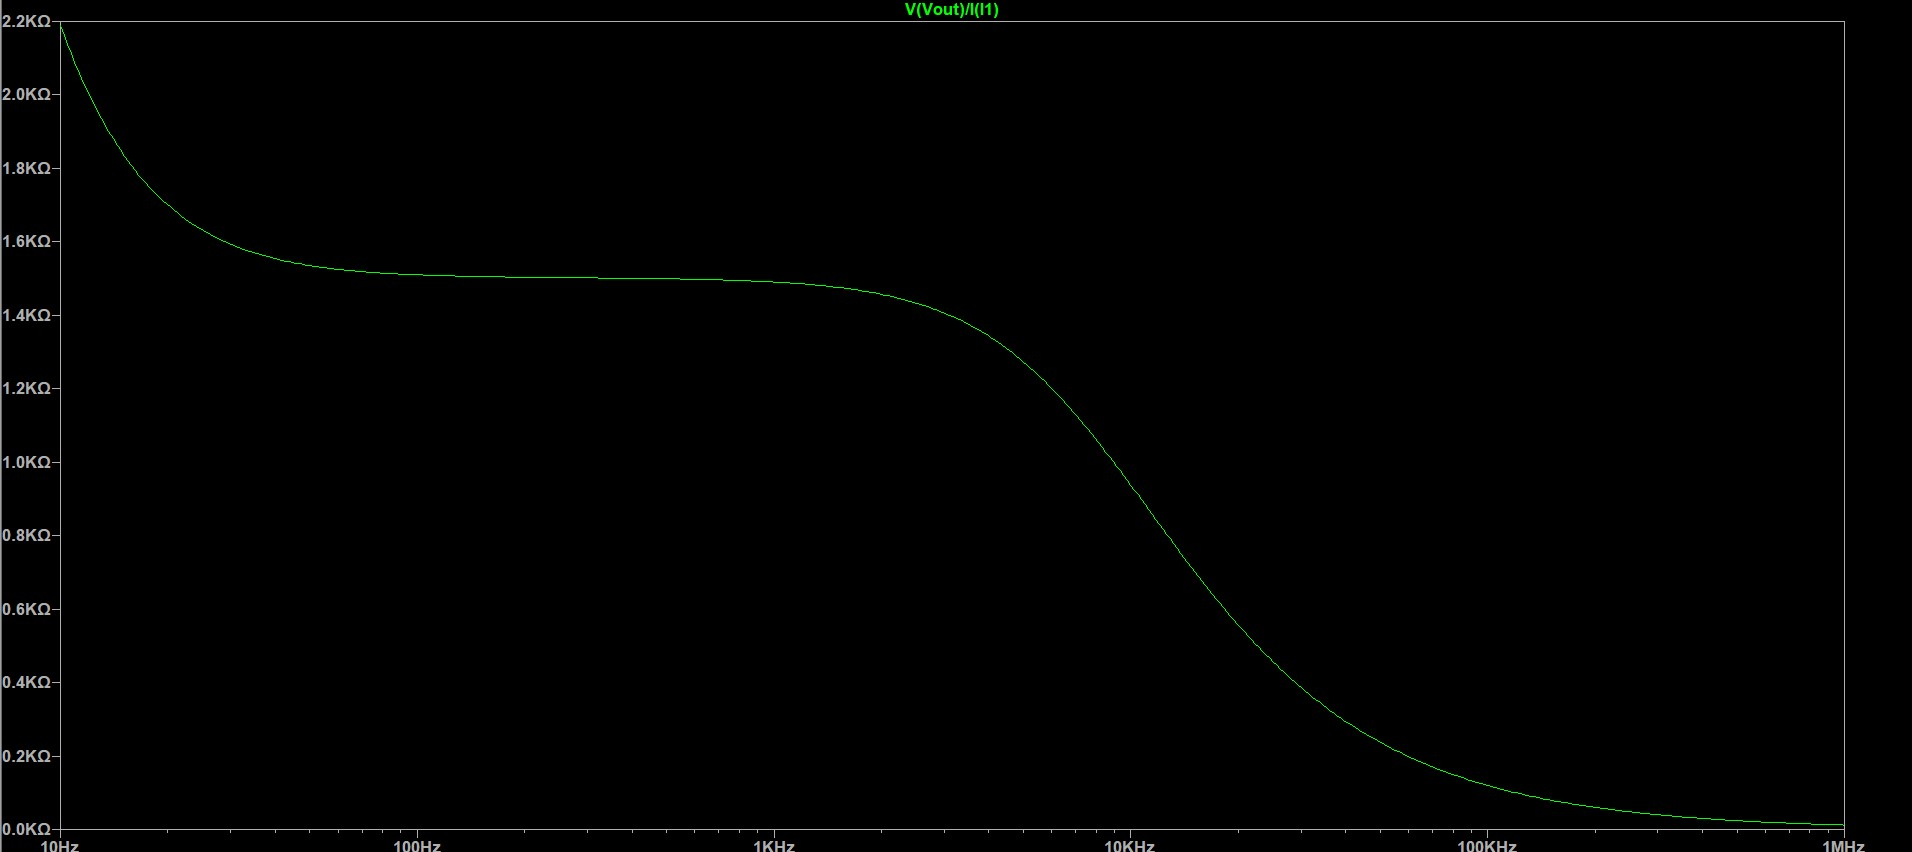
\includegraphics[width=\linewidth]{Simu-Feli/Fotos/Imp_salida_total_bode.jpg}
        \caption{Montaje de medición de la impedancia de salida total $Z_{out}$.}
    \end{minipage}
\end{figure}


% =========================================================================
% APARTADO 2: ETAPA 1
% =========================================================================
\subsection{Primera Etapa del Amplificador MOSFET}

\begin{figure}[H]
    \centering
    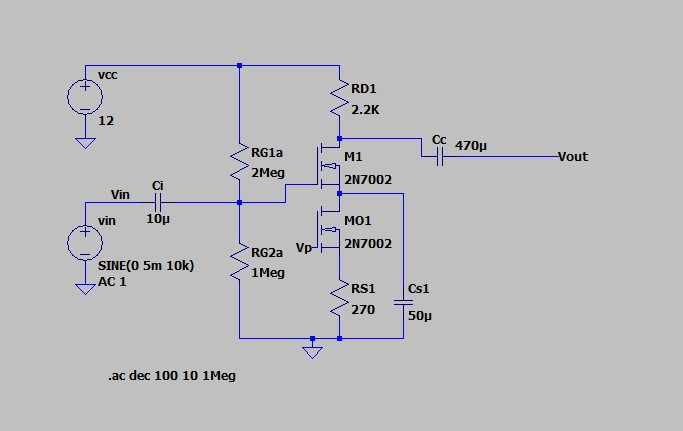
\includegraphics[width=0.55\linewidth]{Simu-Feli/Fotos/Etapa1_Aislada.jpg}
    \caption{Circuito esquemático de la primera etapa aislada.}
\end{figure}

\subsubsection{Ganancia y Ancho de Banda}
\begin{figure}[H]
    \centering
    \begin{minipage}{0.48\textwidth}
        \centering
        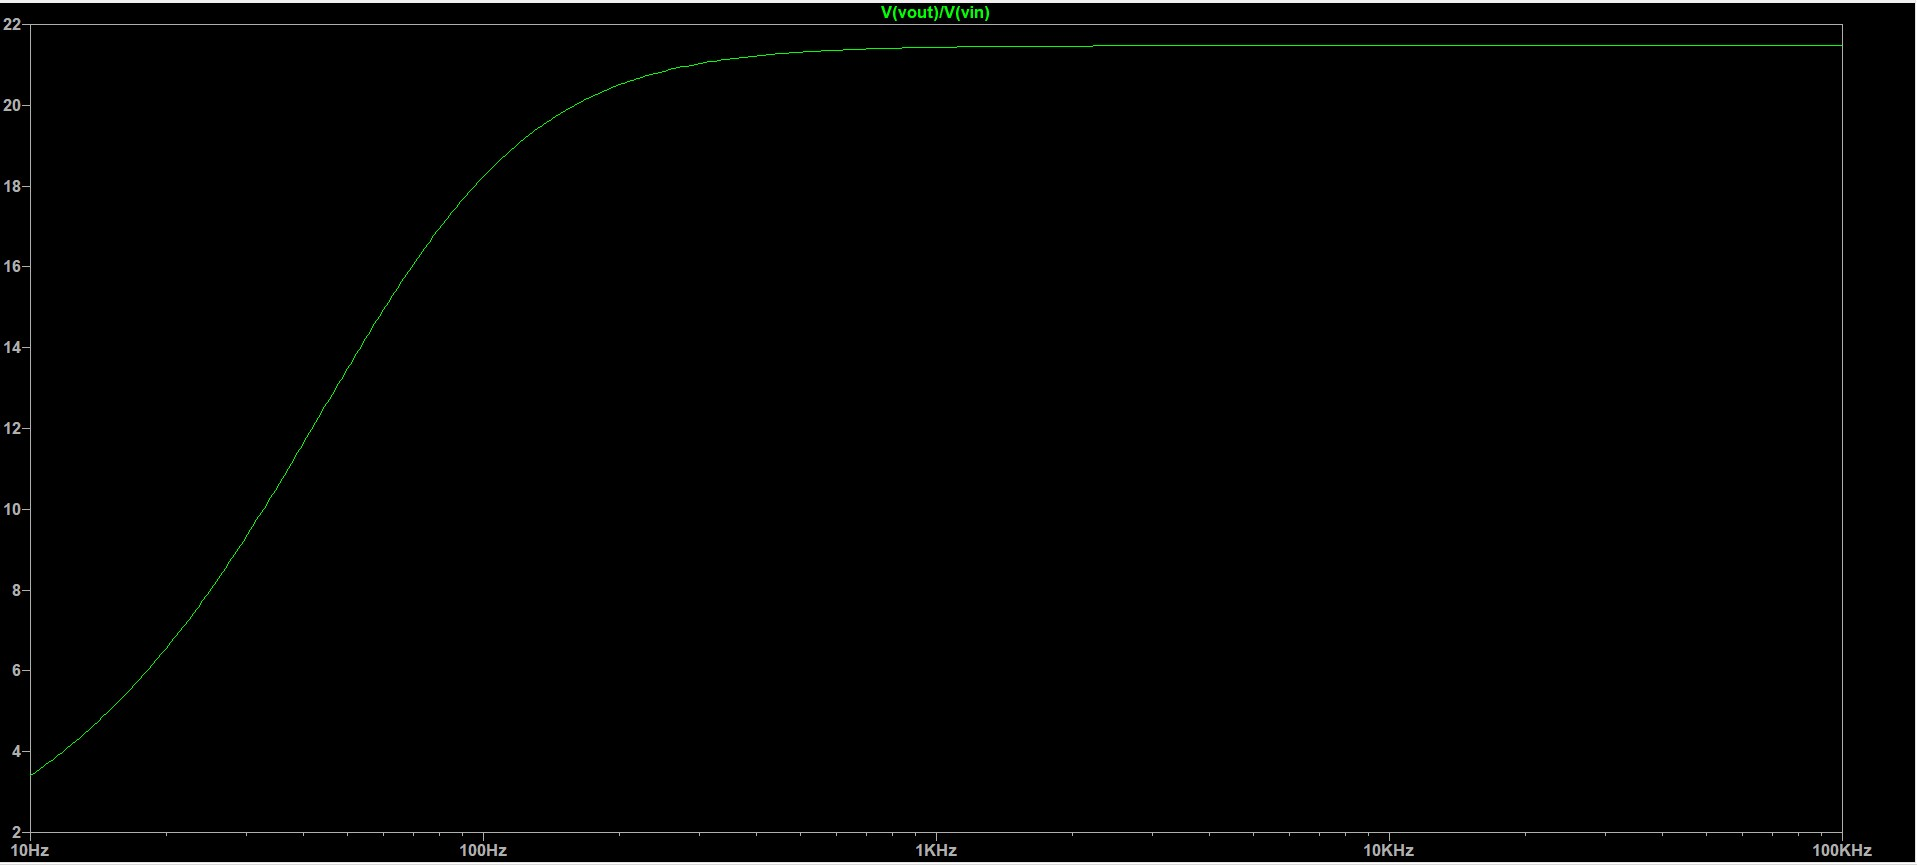
\includegraphics[width=\linewidth]{Simu-Feli/Fotos/Av_Etapa1.jpg}
        \caption{Ganancia de tensión de la etapa 1.}
    \end{minipage}\hfill
    \begin{minipage}{0.48\textwidth}
        \centering
        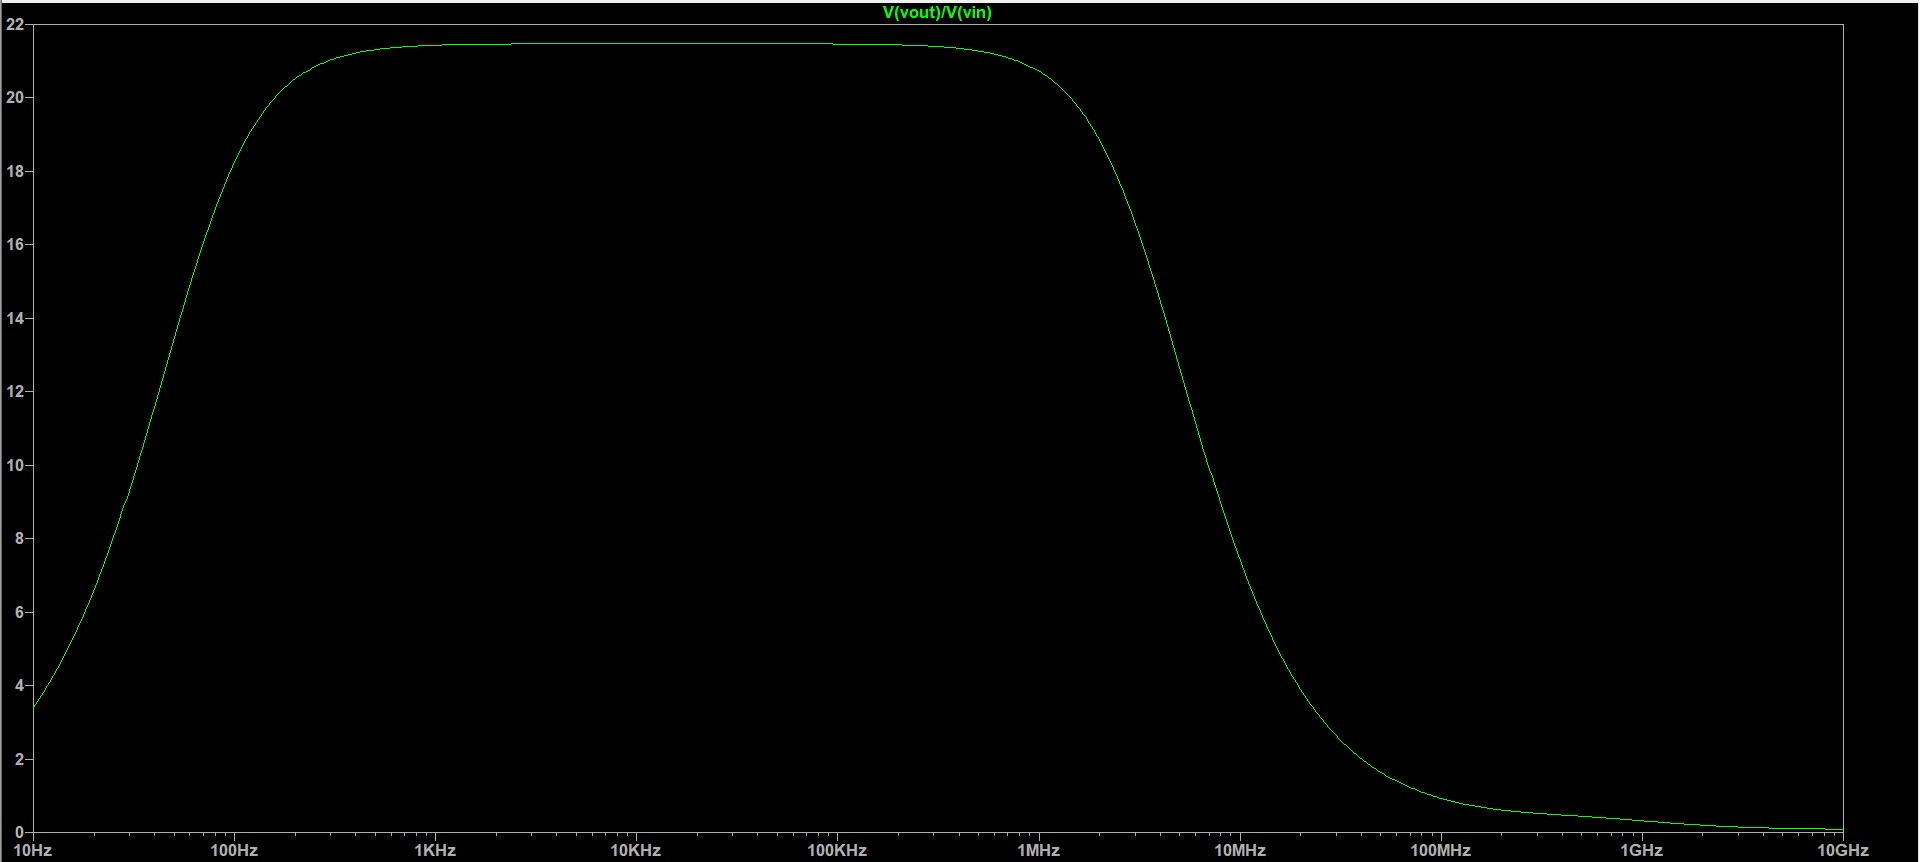
\includegraphics[width=\linewidth]{Simu-Feli/Fotos/Bw_e1.jpg}
        \caption{Ancho de banda de la etapa 1.}
    \end{minipage}
\end{figure}

\subsubsection{Impedancias de la Etapa 1 ($Z_{in1}$ y $Z_{out1}$)}
\begin{figure}[H]
    \centering
    \begin{minipage}{0.48\textwidth}
        \centering
        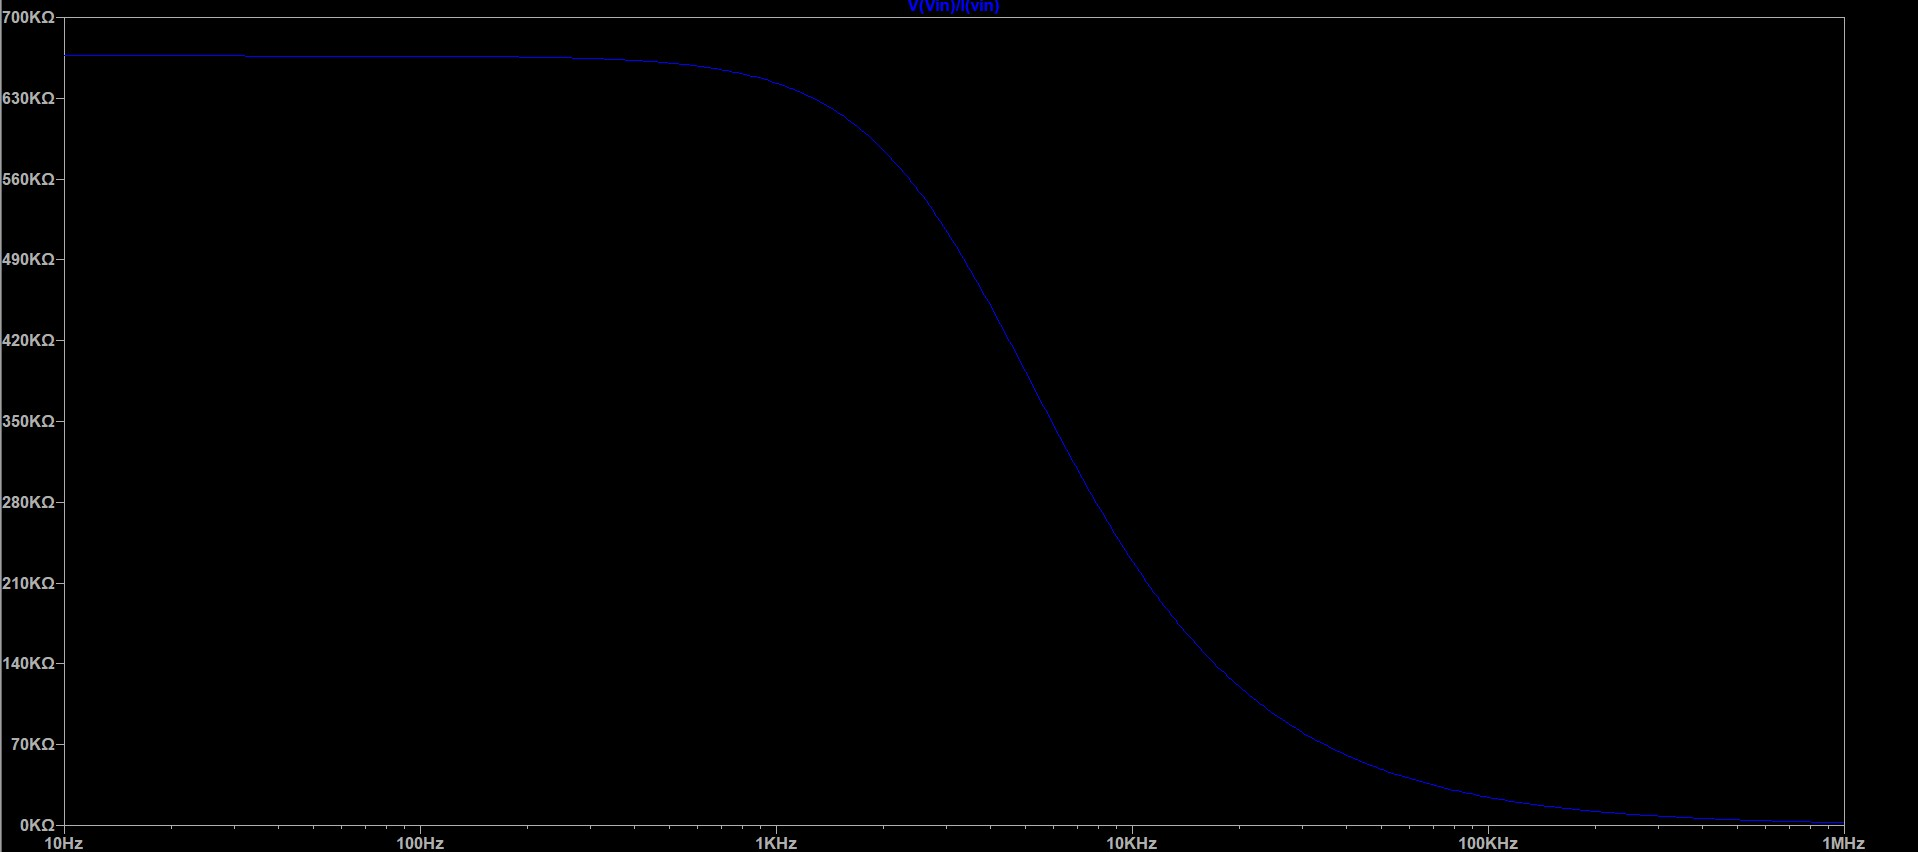
\includegraphics[width=\linewidth]{Simu-Feli/Fotos/Impedancia_In_E1_bode.jpg}
        \caption{Impedancia de entrada $Z_{in1}$.}
    \end{minipage}\hfill
    \begin{minipage}{0.48\textwidth}
        \centering
        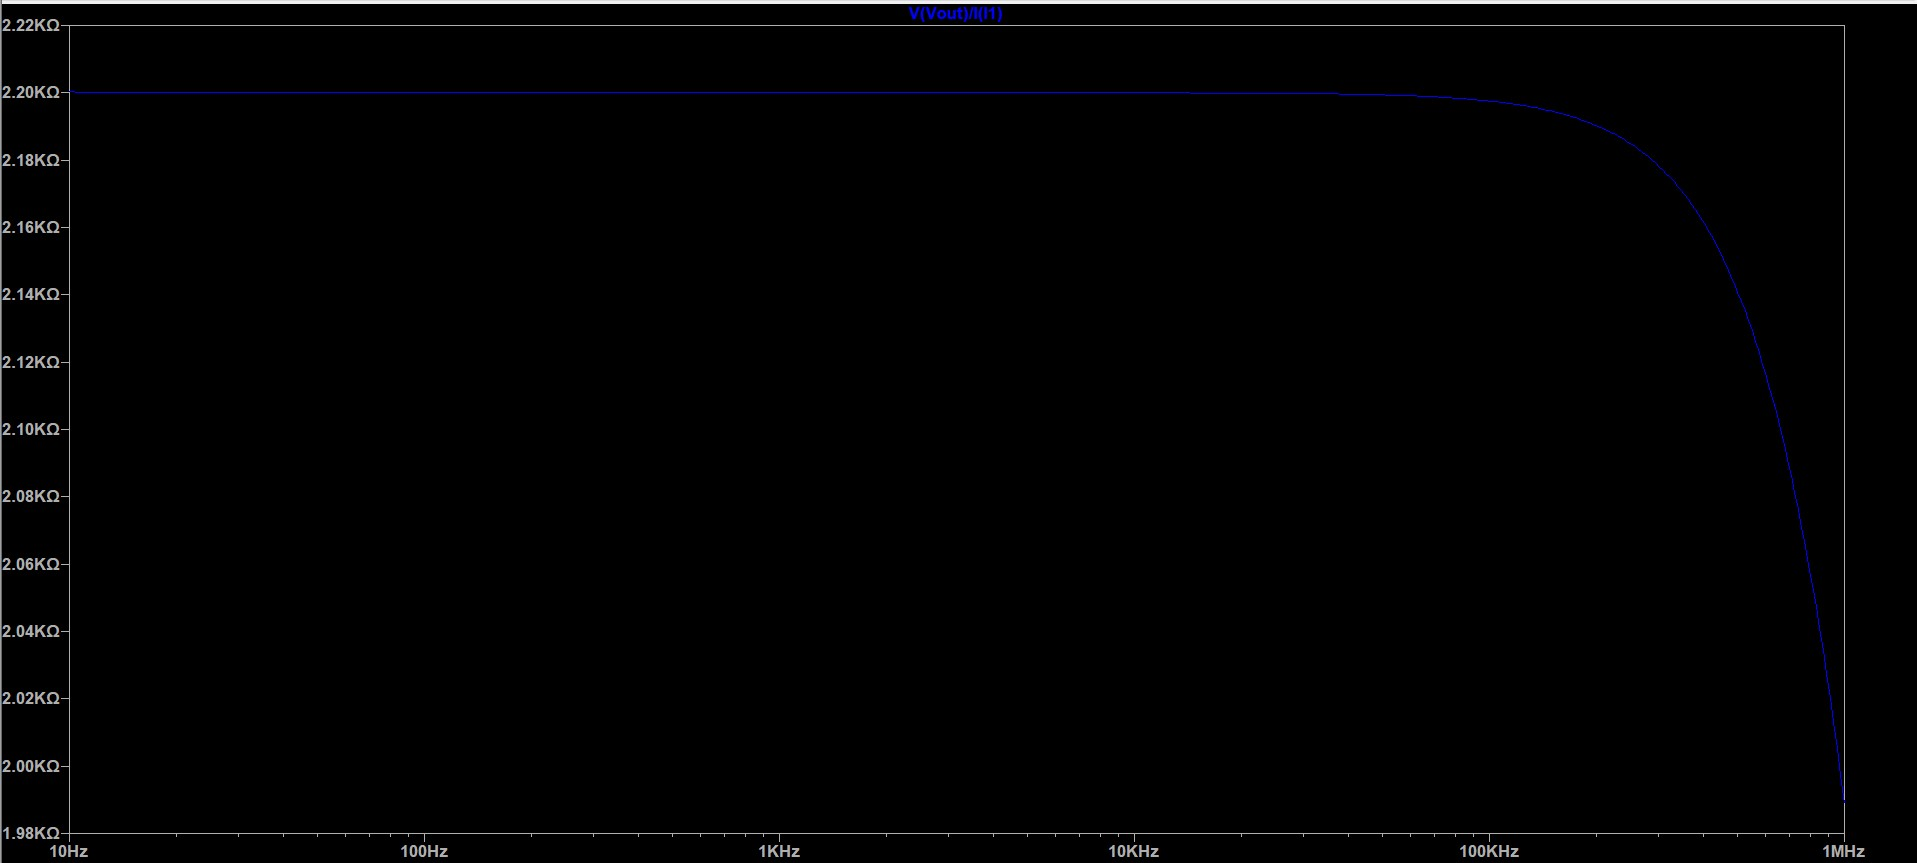
\includegraphics[width=\linewidth]{Simu-Feli/Fotos/Zout_Etapa_1_bode.jpg}
        \caption{Impedancia de salida $Z_{out1}$.}
    \end{minipage}
\end{figure}

% =========================================================================
% APARTADO 3: ETAPA 2
% =========================================================================
\subsection{Segunda Etapa del Amplificador MOSFET}

\begin{figure}[H]
    \centering
    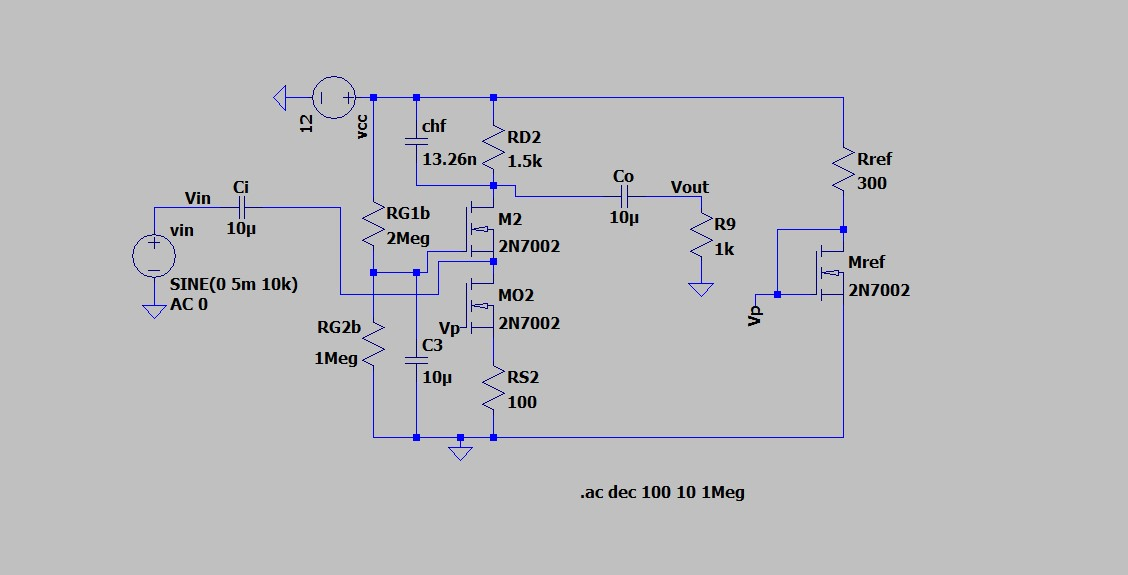
\includegraphics[width=0.55\linewidth]{Simu-Feli/Fotos/Etapa2_Aislada.jpg}
    \caption{Circuito esquemático de la segunda etapa aislada.}
\end{figure}

\subsubsection{Ganancia y Ancho de Banda}
\begin{figure}[H]
    \centering
    \begin{minipage}{0.48\textwidth}
        \centering
        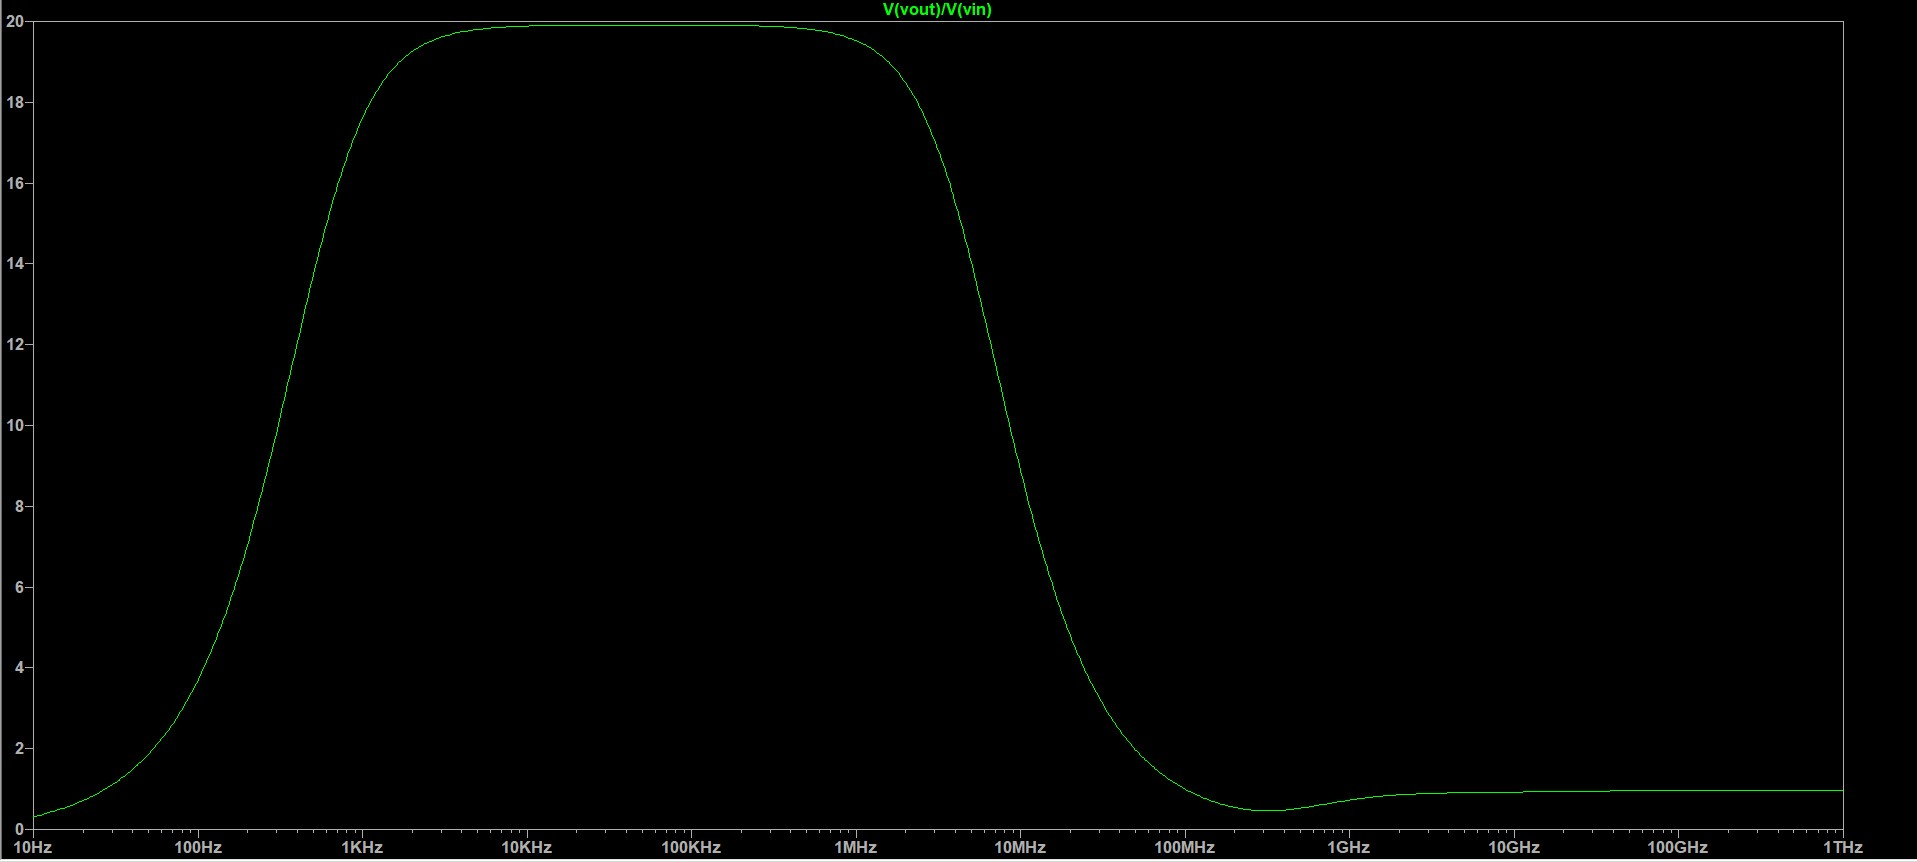
\includegraphics[width=\linewidth]{Simu-Feli/Fotos/AV_Etapa2_sinchf.jpg}
        \caption{Ganancia etapa 2 (sin $C_{hf}$).}
    \end{minipage}\hfill
    \begin{minipage}{0.48\textwidth}
        \centering
        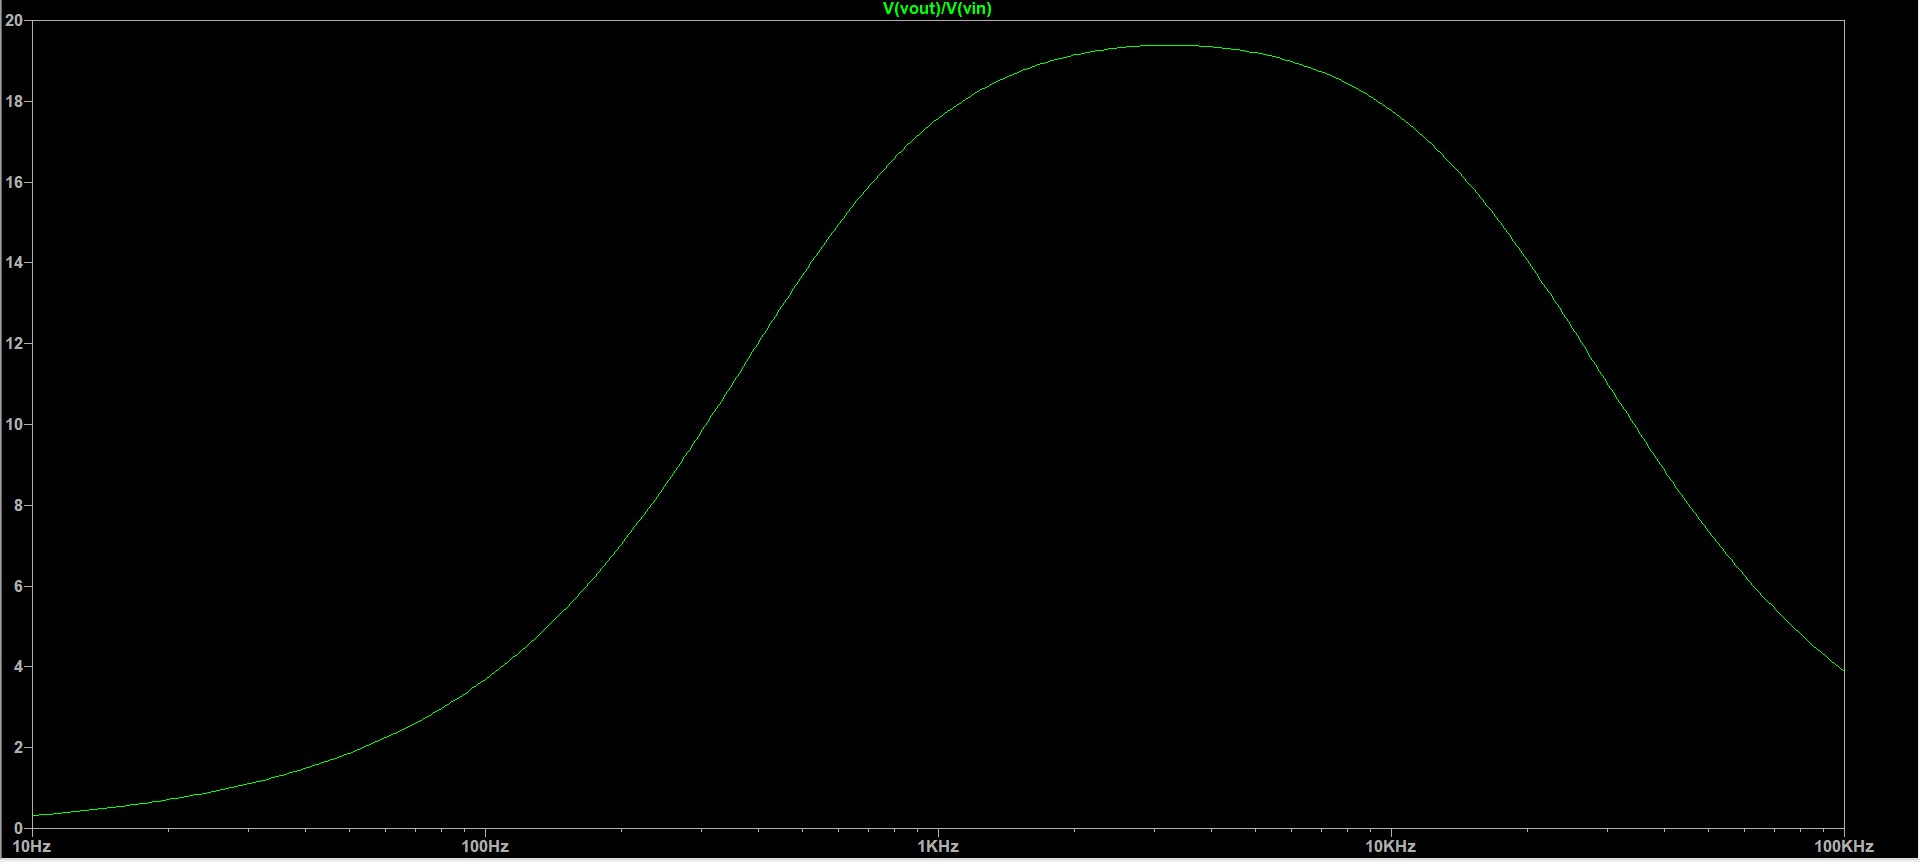
\includegraphics[width=\linewidth]{Simu-Feli/Fotos/Av_Etapa2.jpg}
        \caption{Ganancia etapa 2 general.}
    \end{minipage}
\end{figure}

\subsubsection{Impedancias de la Etapa 2 ($Z_{in2}$ y $Z_{out2}$)}
\begin{figure}[H]
    \centering
    \begin{minipage}{0.48\textwidth}
        \centering
        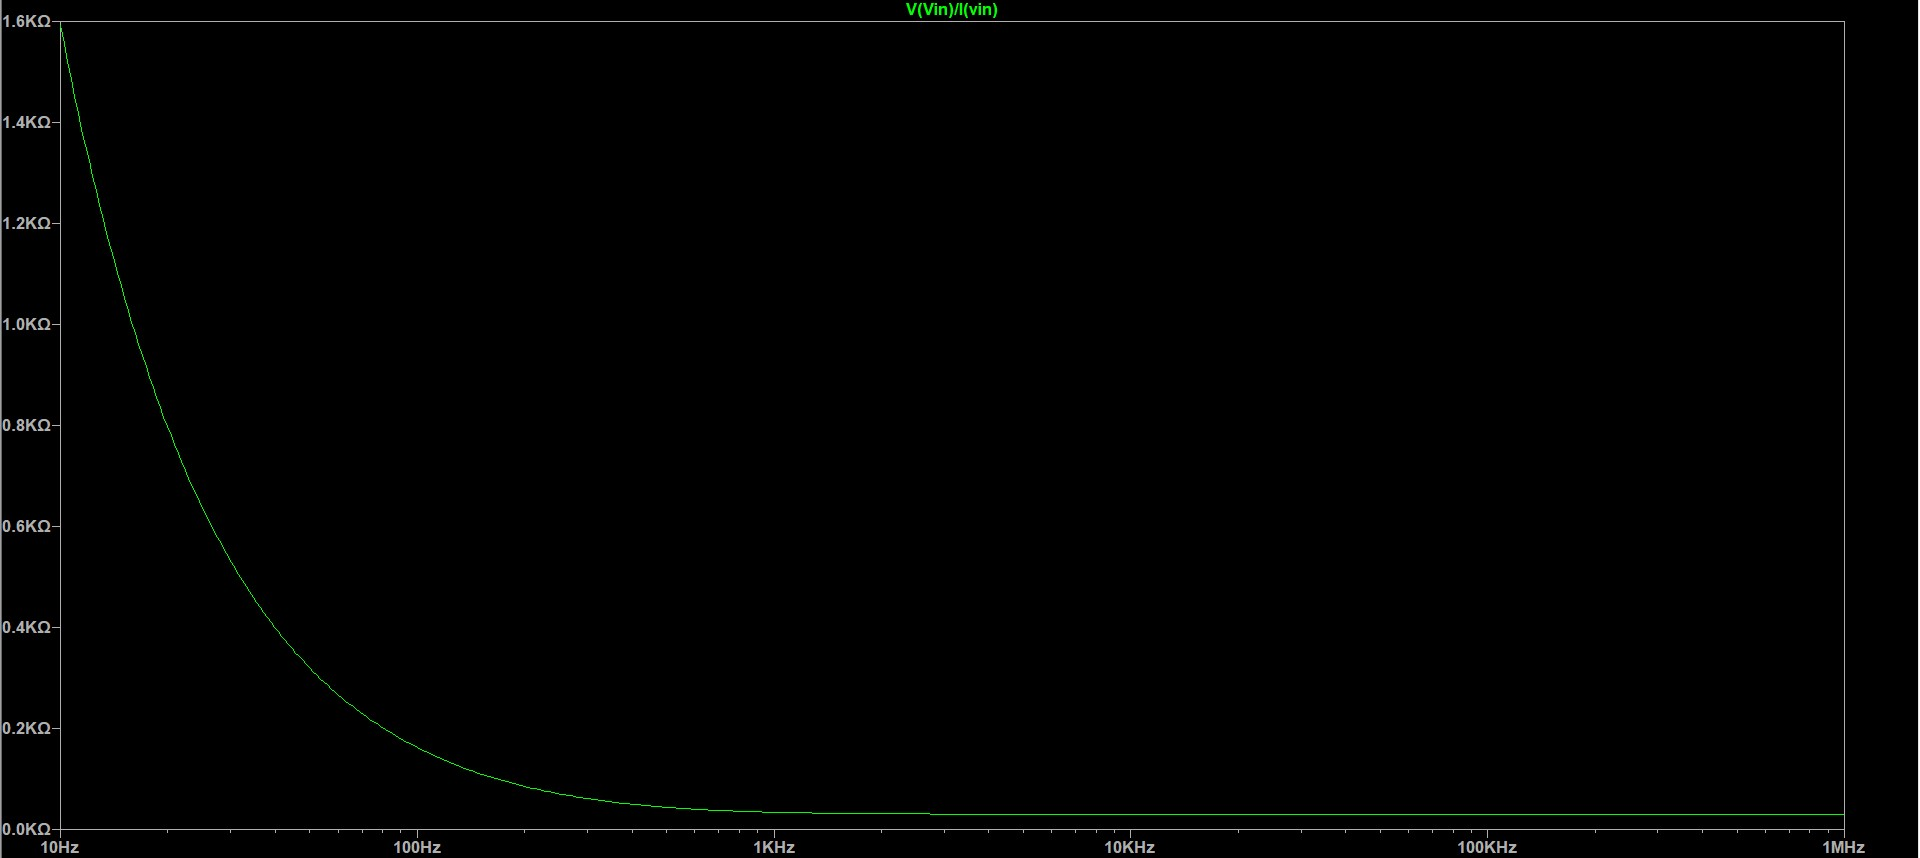
\includegraphics[width=\linewidth]{Simu-Feli/Fotos/Zin_etapa2_bode.jpg}
        \caption{Impedancia de entrada $Z_{in2}$.}
    \end{minipage}\hfill
    \begin{minipage}{0.48\textwidth}
        \centering
        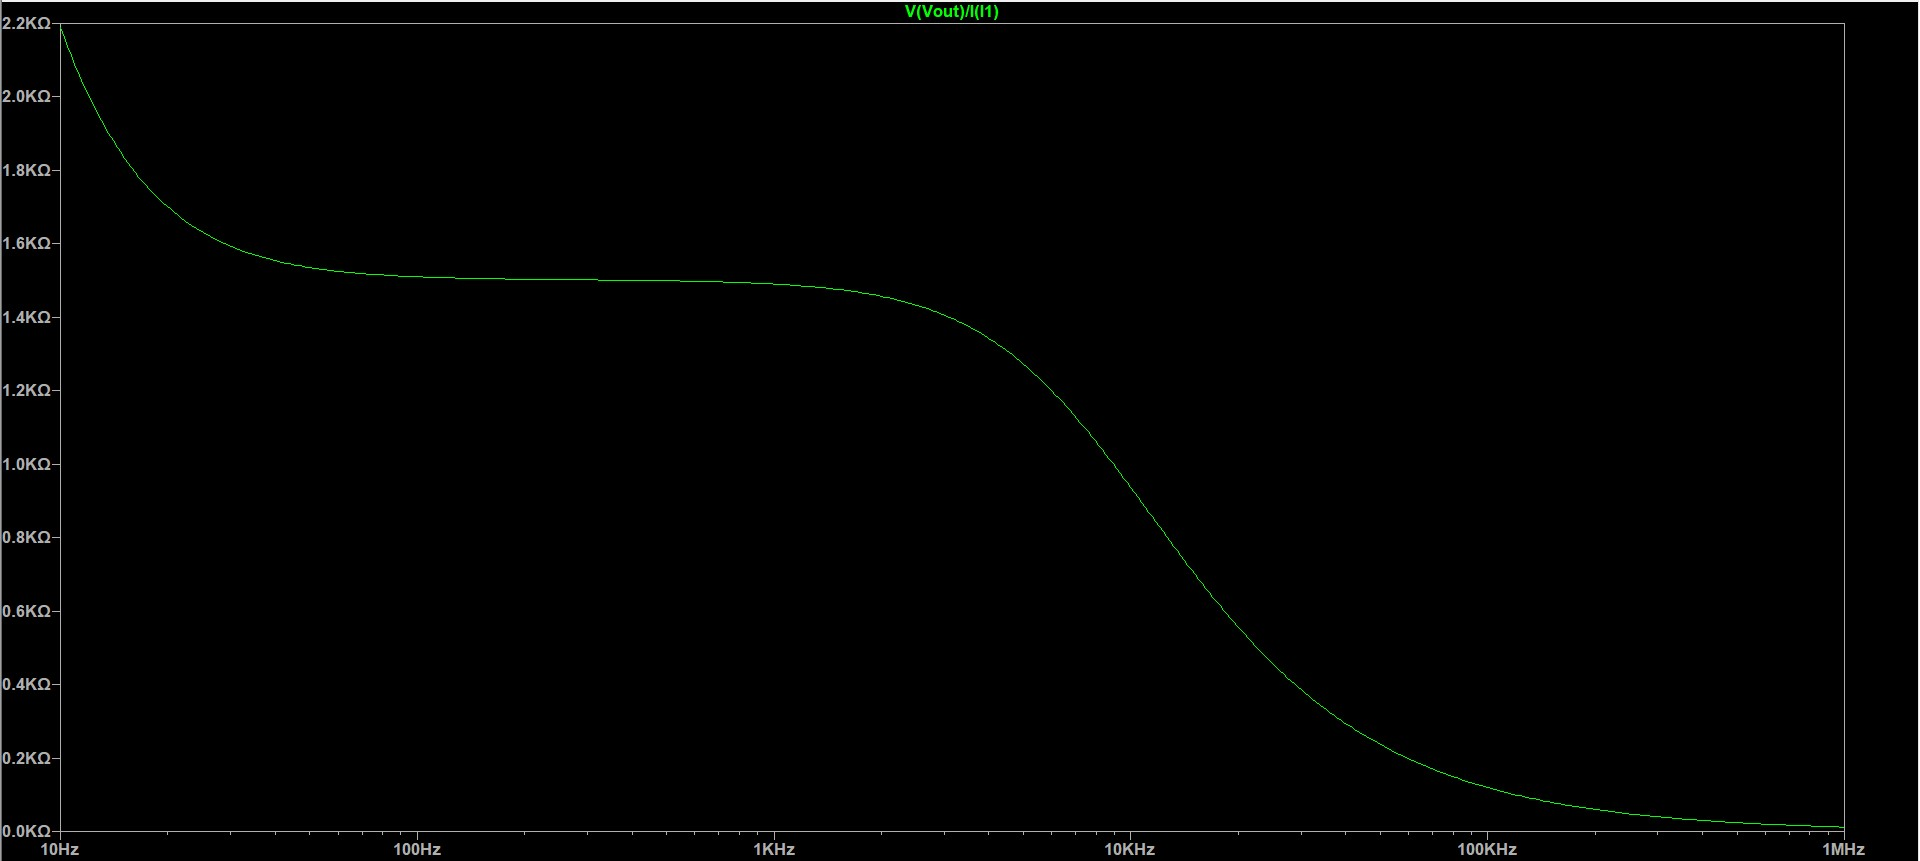
\includegraphics[width=\linewidth]{Simu-Feli/Fotos/Zout_etapa_2_bode.jpg}
        \caption{Impedancia de salida $Z_{out2}$.}
    \end{minipage}
\end{figure}

\subsection{Diseño de PCB}

Para el disenio del circuito en la placa se utilizó el programa KiCAD, se comenzo por su esquematico, tomando de referencia al brindado por la catedra

\begin{figure}[H]
  \centering
  \resizebox{250}{!}
  {
    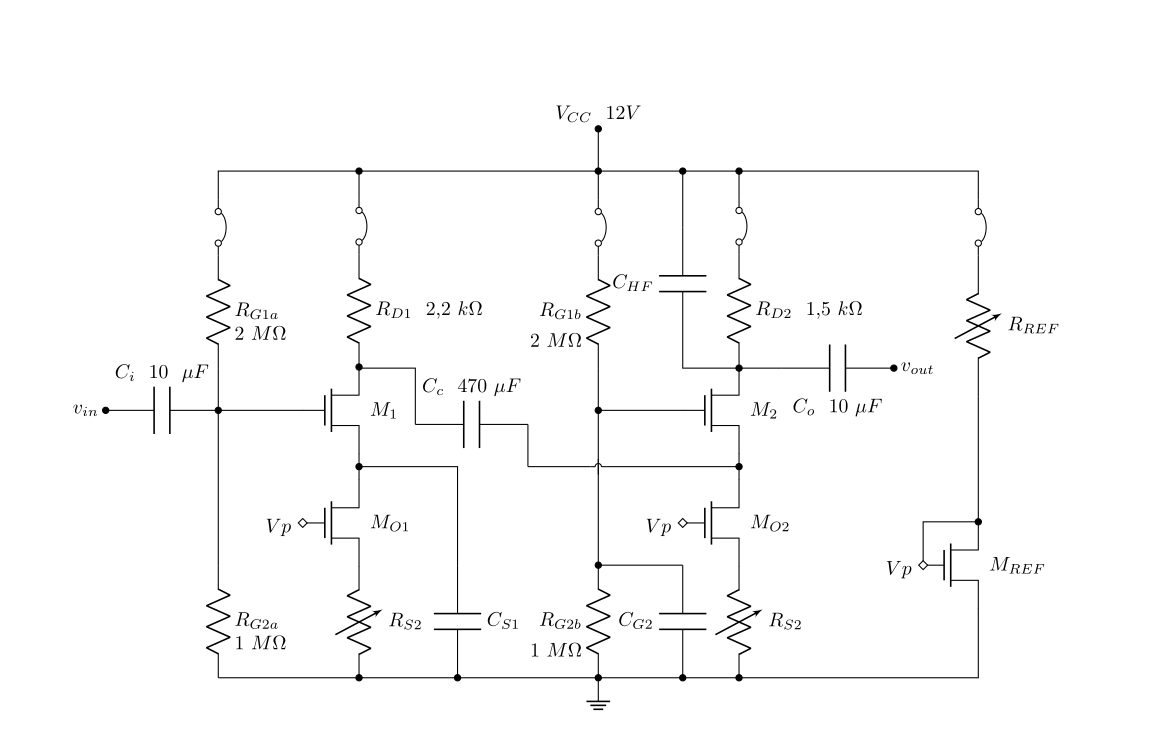
\includegraphics{Imagenes/EsquematicoCatedra.png}
  }
  \caption{Esquemático de la Catedra}
  \label{Esquematico_Cátedra}
\end{figure}

  Adicionalmente a este se le implementaron los siguientes componentes:
\begin{enumerate}
  \item Jumpers de aislación de etapas
  \item Test Points para la mediciones de Tension
  \item Headers macho a 90 grados para conectores BNC de entrada.
  \item Bornera doble de alimentación
  \item Jumpers de Aislacion de Presets
\end{enumerate}

Se tuvieron en cuenta las mediciones de la consigna para posicionar los puntos de prueba en el circuito, se optó por omitir aquellos Test Points en lugares donde los componentes de montaje brinden el espacio para su prueba con el fin de obtener un diseño más compacto y de menor costo.

\vspace{0.5em}
{\small\textbf{Diseño de Esquemático}}

Una vez constituido el esquemático (\ref{Esquematico}) a utilizar se le asignaron las huellas de los componentes, estas fueron designadas según la disipación de potencia estimada y las especifiaciones de MOSFET de la catedra.

\begin{figure}[H]
  \centering
  \resizebox{250}{!}{
    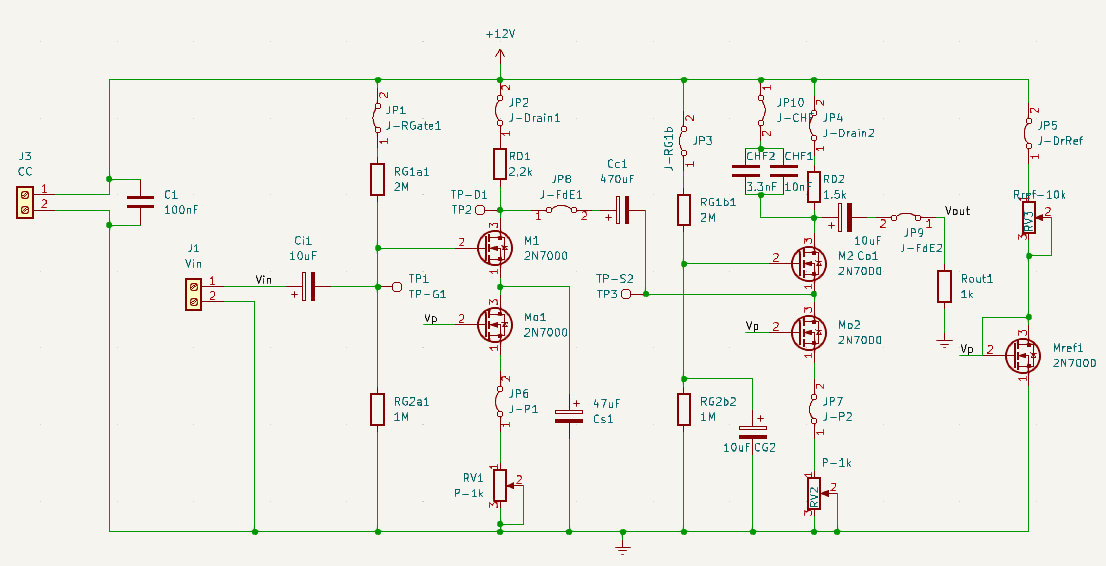
\includegraphics{Imagenes/Esquematico.png}
  }
  \caption{Esquemático del diseño final}
  \label{Esquematico}
\end{figure}

\vspace{0.5em}
{\small\textbf{Diseño de PCB }}

Para el enrutamiento (\ref{fig:trazas}) de los componentes y su disposición se tuvieron en cuenta diversos factores:

\begin{enumerate}
  \item Ancho de vía general: $1_{mm}$
  \item Jumpers en posición horizontal
  \item Polaridad de los header a 90 grados según la bornera BNC
  \item Jumpers ubicados en el exterior de la placa
  \item Plano de GND rodeando el circuito
  \item Conexión de componentes mediante la capa B.Cu (Bottom Copper) 
  \item Zonas de relleno con conexión a tierra, alivios térmicos y separación de contornos de $0.4_{mm}$
  \item Dimensiones de placa $41_{cm^2}$
  \item Posicionamiento de los presets en el exterior de la placa y con orientacion de ranura hacia afuera
  \item Uso de ángulos a 45 grados para evitar la discontinuidad en la impedancia característica de la pista, estrés y el efecto de “Trampa de ácido” por tensión superficial
\end{enumerate}

\begin{figure}[H]
  \centering
  \resizebox{250}{!}
  {
      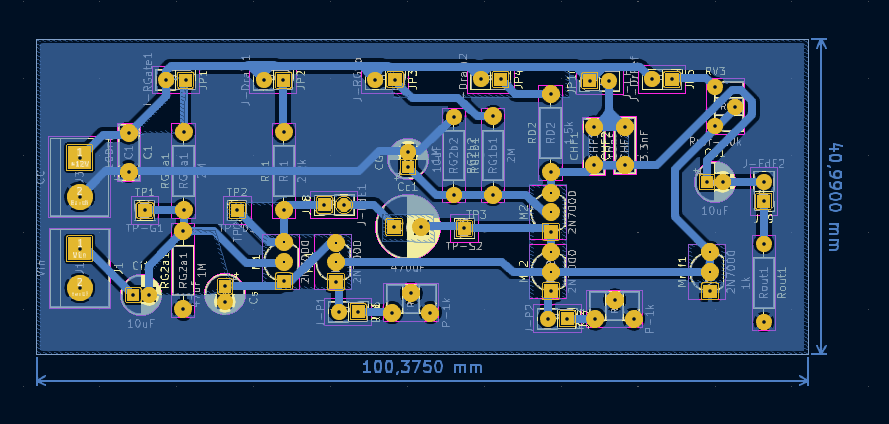
\includegraphics{Imagenes/Trazas.png}
  }
  \caption{Vista del Bottom Copper del diseño}
  \label{fig:trazas}
\end{figure}

\vspace{0.5em}
{\small\textbf{Diseño de Impresión }}

A continuación se presenta el diseño (\ref{fig:impreso}) utilizado para transferir las pistas a la placa de cobre

\begin{figure}[H]
  \centering
  \resizebox{250}{!}
  {
    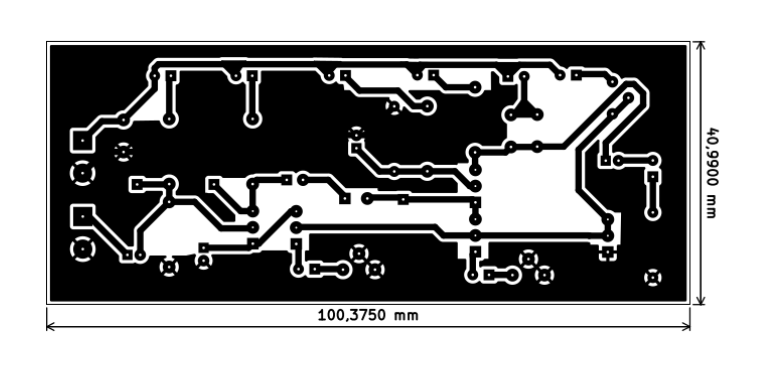
\includegraphics{Imagenes/Impreso.png}
  }
  \caption{Diseño de Impresión final}
  \label{fig:impreso}
\end{figure}

\section{Conclusión}

Se pudo ver en el análisis de los resultados que, si bien el modelo de los transistores utilizado en el diseño difiere del utilizado en la simulación y que estos a su vez son distíntos de los capacitores reales, se obtuvieron resultados satisfactorios en el circuito final.

El parámetro alejado de los requisitos iniciales es la frecuencia de corte en alta frecuencia, que da por debajo del valor calculado y simulado. La causa posible de esto es justamente la diferencia entre los parámetros reales de capacidad parásita del transistor $M_1$, con el que se calculó esta frecuencia, y el valor obtenido de la hoja de datos.


\newpage

\printbibliography
%\bibliographystyle{ieeetr}
%\bibliography{bibliografia}
\end{document}